\section{المقدمة}
\label{sec:introduction}

يركز إخفاء المعلومات اللغوي على التضمين الخفي للمعلومات السرية داخل حوامل نصية تبدو بريئة. وتعتمد المنهجيات التقليدية، القائمة أساسًا على الاستبدال المعجمي والتلاعب بالمرادفات \cite{qiang2023natural}، على قدر محدود من التكرار في اللغة الطبيعية. لذلك يمكن حتى للانحرافات الإحصائية الصغيرة أن تقدم إشارة كافية لأنظمة الكشف الآلي الحديثة \cite{yang2020vae,kaptchuk2021meteor,Wang_2023}. وقد أدى ظهور نماذج اللغة الكبيرة \EN{Large Language Models (LLMs)} إلى تحول في المجال من تعديل النصوص إلى توليد النصوص ابتداءً \cite{li2023rewriting,lin2024zero,wu2024generative}. ومن خلال أخذ العينات مباشرة من التوزيع الاحتمالي المتعلم في النموذج، تستطيع هذه المناهج التوليدية نظريًا تحقيق مستويات عالية من اللامحسوسية الإحصائية.

ومع ذلك، تبقى أنظمة إخفاء المعلومات المعتمدة على نماذج اللغة الكبيرة مقيدة بمفاضلة أساسية بين الأمن الإحصائي والطبيعية الإدراكية \cite{lin2024zero,wu2024generative,li2023rewriting}. فقد ينتج النموذج جملًا سليمة نحويًا وإحصائيًا، لكنها تفتقر غالبًا إلى الاتساق الدلالي العميق المطلوب لسياقات تواصلية محددة، مثل نقاشات وسائل التواصل الاجتماعي المتسلسلة \cite{liao2024co,wang2023hi,zhang2024controllable}. فالتعليق المتقن لغويًا لكنه غير ملائم تداوليًا لمسار النقاش يصبح شذوذًا واضحًا عند الفحص البشري أو الدلالي.

ولمعالجة هذه التحديات، نقدم إطارًا لإخفاء المعلومات واعيًا بالسياق يرفع مجال التضمين من المستوى المعجمي، أي الرموز الفردية، إلى المستوى الدلالي، أي قرارات المحادثة. فبدلًا من التلاعب بتوزيعات الرموز، يحمل مخططنا الحمولة عبر \textit{قناة اختيار}: حيث تقابل البتات (1) فهرس هدف الرد ضمن شجرة تعليقات مسطحة حتميًا، و(2) فهرس \textit{استطرادة} مشروطة بالسياق ضمن مجموعة استطرادات مشتركة يعيد الطرفان بناءها حتميًا من السلسلة العامة والبحث القابل للإعادة. ثم يولد نموذج اللغة ردًا مرئيًا عاديًا يعمل بوصفه \textit{شاهدًا قابلًا لفك الترميز} على الاستطرادة المختارة؛ ولا نعتمد على محارف غير مرئية أو محارف تحكم في \EN{Unicode}. وتغلق حلقة تحقق من جانب المرسل النظام عبر محاكاة فك الترميز لدى المستقبل قبل النشر. يبين الشكل~\ref{fig:token-vs-intent} الفرق بين التضمين على مستوى الرموز والتضمين ثنائي الطبقة عبر قناة الاختيار في نقاش متسلسل.

\begin{figure}[t]
	\centering
	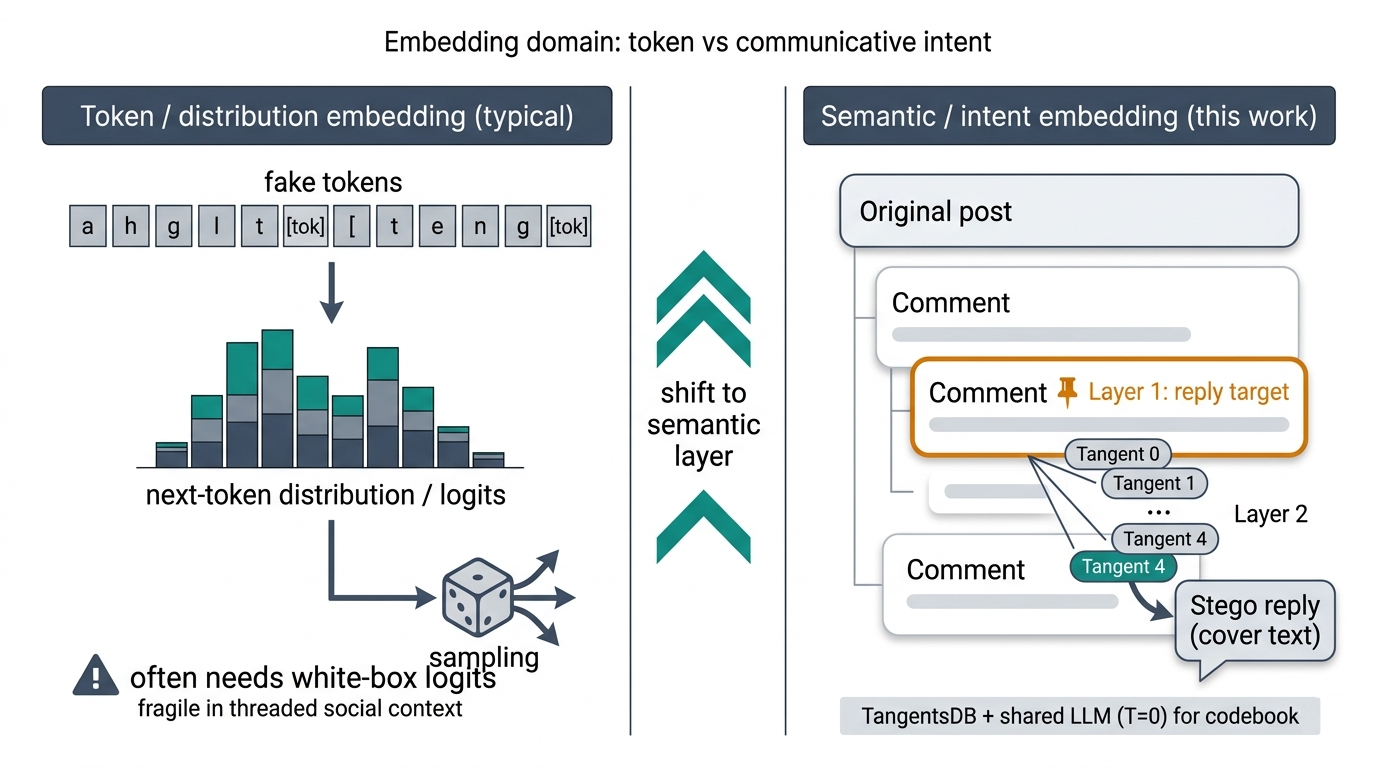
\includegraphics[width=0.78\linewidth]{figures/token_vs_intent_embedding}
	\caption{مقارنة مفهومية بين التضمين على مستوى الرموز والتضمين الدلالي ثنائي الطبقة المقترح فوق نقاش متسلسل.}
	\label{fig:token-vs-intent}
\end{figure}

تتمثل المساهمات الرئيسة لهذه الورقة في الآتي:
\begin{itemize}
    \item بنية تضمين ثنائية الطبقة عبر قناة اختيار للنقاشات المتسلسلة، ترمز البتات في استهداف الرد واختيار الاستطرادة، ويعمل النص المرئي فيها شاهدًا قابلًا لفك الترميز لا حاملًا مخفيًا.
    \item خط إعادة بناء حتمي، يجمع السلسلة والبحث القابل للإعادة، يتيح تماثل المرسل والمستقبل دون وصول \EN{white-box} إلى النموذج أو تبادل بيانات وصفية عبر قناة جانبية.
    \item آلية تحقق مغلقة الحلقة تحاكي فك الترميز قبل النشر وتعيد محاولة التوليد لتحسين قابلية الاسترجاع تحت التوليد العشوائي.
\end{itemize}
